\chapter{Design}
The system design is specified in this chapter. The first section illustrates the system architecture, and how the different layers in the system interact on a top-level. The last section is a detailed description of how the main modules in the system should behave.
%structur og modulering i design 

\section{System Architecture}
The blockchain layer and the application layer design are both illustrated in this section. The interaction between the layers is illustrated at the end of the section.
\subsection{Blockchain Layer}
The relation between the modules of the blockchain layer can be seen in figure \ref{fig:blockchain}. The main modules of the system are the \textit{node}, \textit{consensus} and, \textit{network} modules. Whereas the \textit{storage},\textit{messages}, and \textit{block} modules are helper modules. The \textit{node} object in the \textit{node} module is a subclass of the \textit{PeerManager} in the \textit{network} module, which allows the \textit{node} object to directly use methods in the \textit{network} module to communicate with other nodes. 

\begin{figure}[!htb]
\centering
	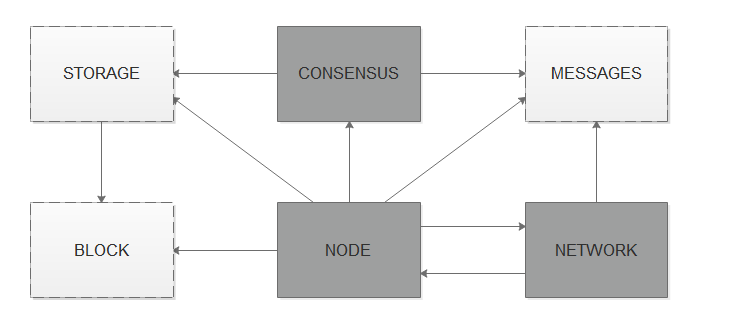
\includegraphics[width=1\textwidth]{Images/blockchain_layer}
	\caption{Connection between modules in blockchain layer.}
	\label{fig:blockchain}
\end{figure}

\subsection{Application Interaction with Blockchain}
\begin{figure}[!htb]
\centering
	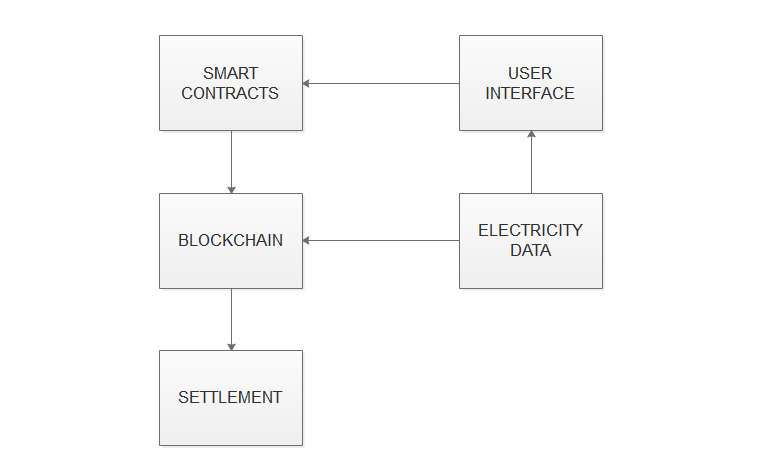
\includegraphics[width=1\textwidth]{Images/application-blockchain}
	\caption{Interaction between application and blockchain.}
	\label{fig:app_blockchain}
\end{figure}

\section{Module Design}
The individual modules in each of the are explained in further detail in this section.
\subsection{Smart Contract}\label{smart}
When a consumer and prosumer initiate a smart contract, the terms of the contract must include the following.
\begin{enumerate}
\item The start time of the contract.
\item The end time of the contract.
\item The ID's of the prosumer and consumer.
\item The minimum amount of electricity transacted between the parties of the contract.
\item Digital signatures from both parties of the contract.
\end{enumerate}

All smart contracts are stored in their own blockchain to increase read efficiency. The contracts are verified with the public keys of the nodes, before it is stored in the blockchain.

The smart contract API is callable from the website, and is triggered when two parties initiate the contract. Any node in the system can only have one active contract at a time. New transactions trigger settlement based on smart contract.

\subsection{Blockchain}
There are two blockchains for the microgrid, one for storing all electricity transactions in the system, and one for storing all smart contracts. The blockchains are the back-end services that enable the settlement process. The purpose of the blockchain is that two different parties cannot claim the same unit of produced energy, or the transaction payment.

\subsection{Settlement} \label{settlement_1}
When the system receives information of consumed and produced electricity of a node, the smart contract is self-enforcing in the manner that these events trigger functions that control the settlement. 

Energy trading is a very complex task, thus four assumptions are made for the settlement module in this system:
\begin{itemize}
\item During any interval, the amount of electricity consumed in the system equals the amount of electricity produced in the system.
\item Any participant in the network has one, and only one, contract with another participant in the system at any given time.
\item If the consumer of a contract has consumed more electricity than the producer of the contract has produced, the excess consumed electricity is produced by the pure producers in the system.
\item If a prosumer produces more electricity than is consumed by itself or the consumer in the contract, during an interval, it is assumed that the electricity is stored in batteries and not part of the settlement process.
\end{itemize}


If prosumer A has a smart contract with consumer B, and the system registers that these nodes have produced and consumed electricity during any interval in the duration of the contract, node B's bill will register that it owes node A for the consumed electricity of the period, and likewise node A's bill will show that node B owes money for the electricity. Each node in the system has a bill of how much the node owes other nodes in the system, and how much other nodes owe this node. The bills are accumulative and assumed settled at regular intervals, e.g. each month.

\subsection{Consensus}
The consensus protocol is modeled after the Raft protocol. Five nodes are in charge of the consensus process in the consortium blockchains. The reason why only five nodes should participate in the consensus process is to reduce the message overhead in the system. The consensus process has a randomly selected leader. Any node can be part of the consensus process, and any node can become leader. If a node participating in the consensus goes offline for some reason, another node will take its place. Nodes in the system send their transactions and contracts to the consensus leader, who then initiates the validation process by creating a block. If consensus is reached among the validating nodes, the block is stored in one of the blockchains, depending on if it contains electricity transaction or a smart contract.
%Send transactions to leader and all other nodes to verify authentication of transactions - assume smart meters are tamper proof

\subsection{Website}
The website is the user interface to the system. A user is either a prosumer or a consumer in the microgrid, or the special case of a super user, who can access all the information of the system. Users may log in to their own profile to monitor real-time, and past, consumption and production of electricity. The log in is done with the user's public and private keys. The website has a trading platform where prosumers advertise how much electricity they are selling. Consumers can inquire the prosumers to make a contract. The contract is finalized and sent to the consensus leader when both parties have signed the contract with their private keys.
